\documentclass[11pt, a4paper]{article}
\usepackage[utf8]{inputenc}
\usepackage{fullpage}
\usepackage{graphicx}
\usepackage{markdown}
\usepackage{mathtools}
\usepackage{wrapfig}
\usepackage{tabu}
\usepackage{colortbl}
\usepackage[hidelinks]{hyperref,xcolor}
\usepackage[backend=biber]{biblatex}
\usepackage{adjustbox}
\usepackage{nomencl}
\renewcommand\UrlFont{\color{blue}\rmfamily}
\addbibresource{projectplan.bib}
\addbibresource{prr.bib}
\addbibresource{frr.bib}

\title{Final Research Report\\Remote Water Sensing using UAVs}
\author{Robin \textsc{Westerik}}
\newcommand{\supervisors}{Jan \textsc{Bollen}\\Harry \textsc{Futselaar}}

\newcommand{\timePeriod}{February 2022 - June 2022}
\newcommand{\sprint}{Research}
\newcommand{\homepage}{\url{https://github.com/organizations/remotewatersensing/}}
\date{\today}

\makeatletter{}

\makenomenclature
\renewcommand{\nomname}{}

\begin{document}

\begin{titlepage}
  	\newcommand{\HRule}{\rule{\linewidth}{0.3mm}}
	\center
	\textsc{\LARGE Saxion University of Applied Sciences}\\[1.5cm]
	\textsc{\Large International Water Technology}\\[0.5cm]
	\textsc{\large Applied Computer Science Graduation Project}\\[0.5cm]
	\HRule\\[0.4cm]
	{\huge\bfseries \@title}\\[0.4cm]
	\HRule\\[1.5cm]

	%Author(s)
	\begin{minipage}{0.4\textwidth}
		\begin{flushleft}
			\large
			\textit{Author(s)}\\
			\@author % Your name
		\end{flushleft}
	\end{minipage}
	~
	\begin{minipage}{0.4\textwidth}
		\begin{flushright}
			\large
			\textit{Supervisor(s)}\\
			\supervisors
		\end{flushright}
	\end{minipage}
	
% 	If you don't want a supervisor, uncomment the two lines below and comment the code above
% 	{\large\textit{Author(s)}}\\
% 	\@author % Your name

	%Date
	\vfill\vfill
		{\large\today}
    \vfill\vfill
    
    \footnotesize{Time period: \timePeriod}
    \\[0.3cm]
    \footnotesize{Sprint: \sprint}
    \vfill
    \homepage
    
    \vfill
    
    \begin{tabular}{ | l | l | l | l |}
    \hline
    \textbf{Version} & \textbf{Date of change} & \textbf{What is changed?} & \textbf{The reason for the change} \\ \hline
    0.1 & 17-05-2022 & templating & \\
    0.2 & 17-05-2022 & acidity & \\
    0.3 & 18-05-2022 & conductivity temperature & \\
    
    \hline
\end{tabular}
	
	\vfill\vfill
	
\includegraphics[width=0.4\textwidth]{./saxionlogo.png}
	\vfill
	 
	\vfill
	
\end{titlepage}

\nomenclature{\(FS\)}{Full-Scale}

\tableofcontents
\pagebreak

\section{Abbreviations}
\sffamily\footnotesize
\printnomenclature
\rmfamily\normalsize

\section{Introduction}

In this final research report, the designed prototypes will be tested on several quantitative and qualitative features will be tested. These
features include accuracy, speed, and cost. 

\newpage
\section{Sensors}

The sensor package on the drone is equipped with a turbidity, conductivity, and acidity meter. A minimum accuracy and range requirement for these sensors will be established based on an use case provided by PERNAM JSC. Accuracy of these parameters will be measured both in the laboratory and in practice. All sensors are calibrated accordingly beforehand.

\subsection{Acidity} \label{sensors:acidity}

As mentioned in the Design Report, the DFRobot SEN0169 V2 Pro \cite{SEN0169V2} was chosen for measuring the acidity. The manufacturer claims the sensor has a resolution of 0.1pH across the whole range from 0 to 14pH.\\

The chosen sensor was compared against the Hanna pHep, that also has a resolution of 0.1pH. \cite{hanna} Two solutions with different pH were tested on both sensors

\begin{figure}[h]
  \centering
  \begin{minipage}[b]{0.4\textwidth}
    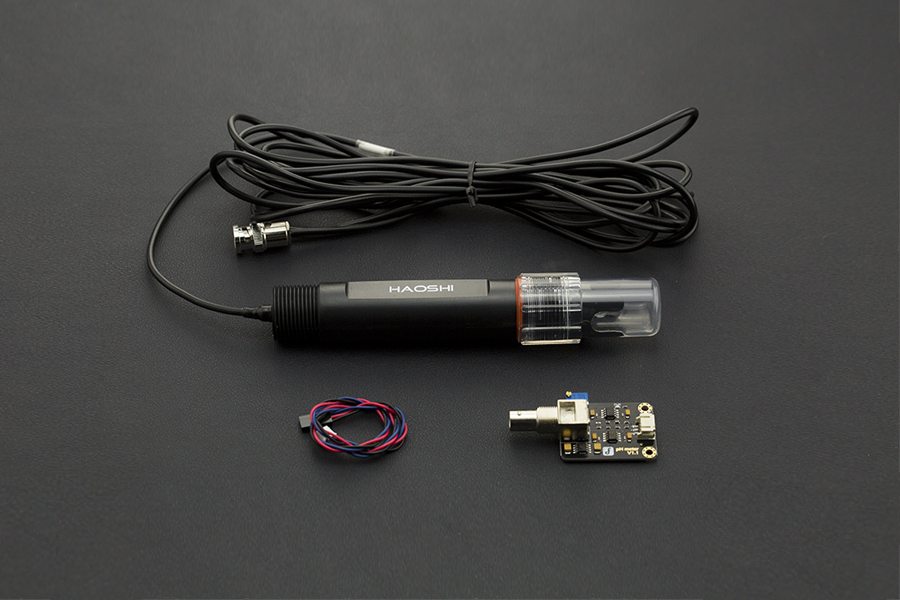
\includegraphics[width=\textwidth]{sensors/12_gravityv2pro.jpg}
    \caption{SEN0169 V2 Pro \cite{SEN0169V2}}
  \end{minipage}
  \hfill
  \begin{minipage}[b]{0.3\textwidth}
    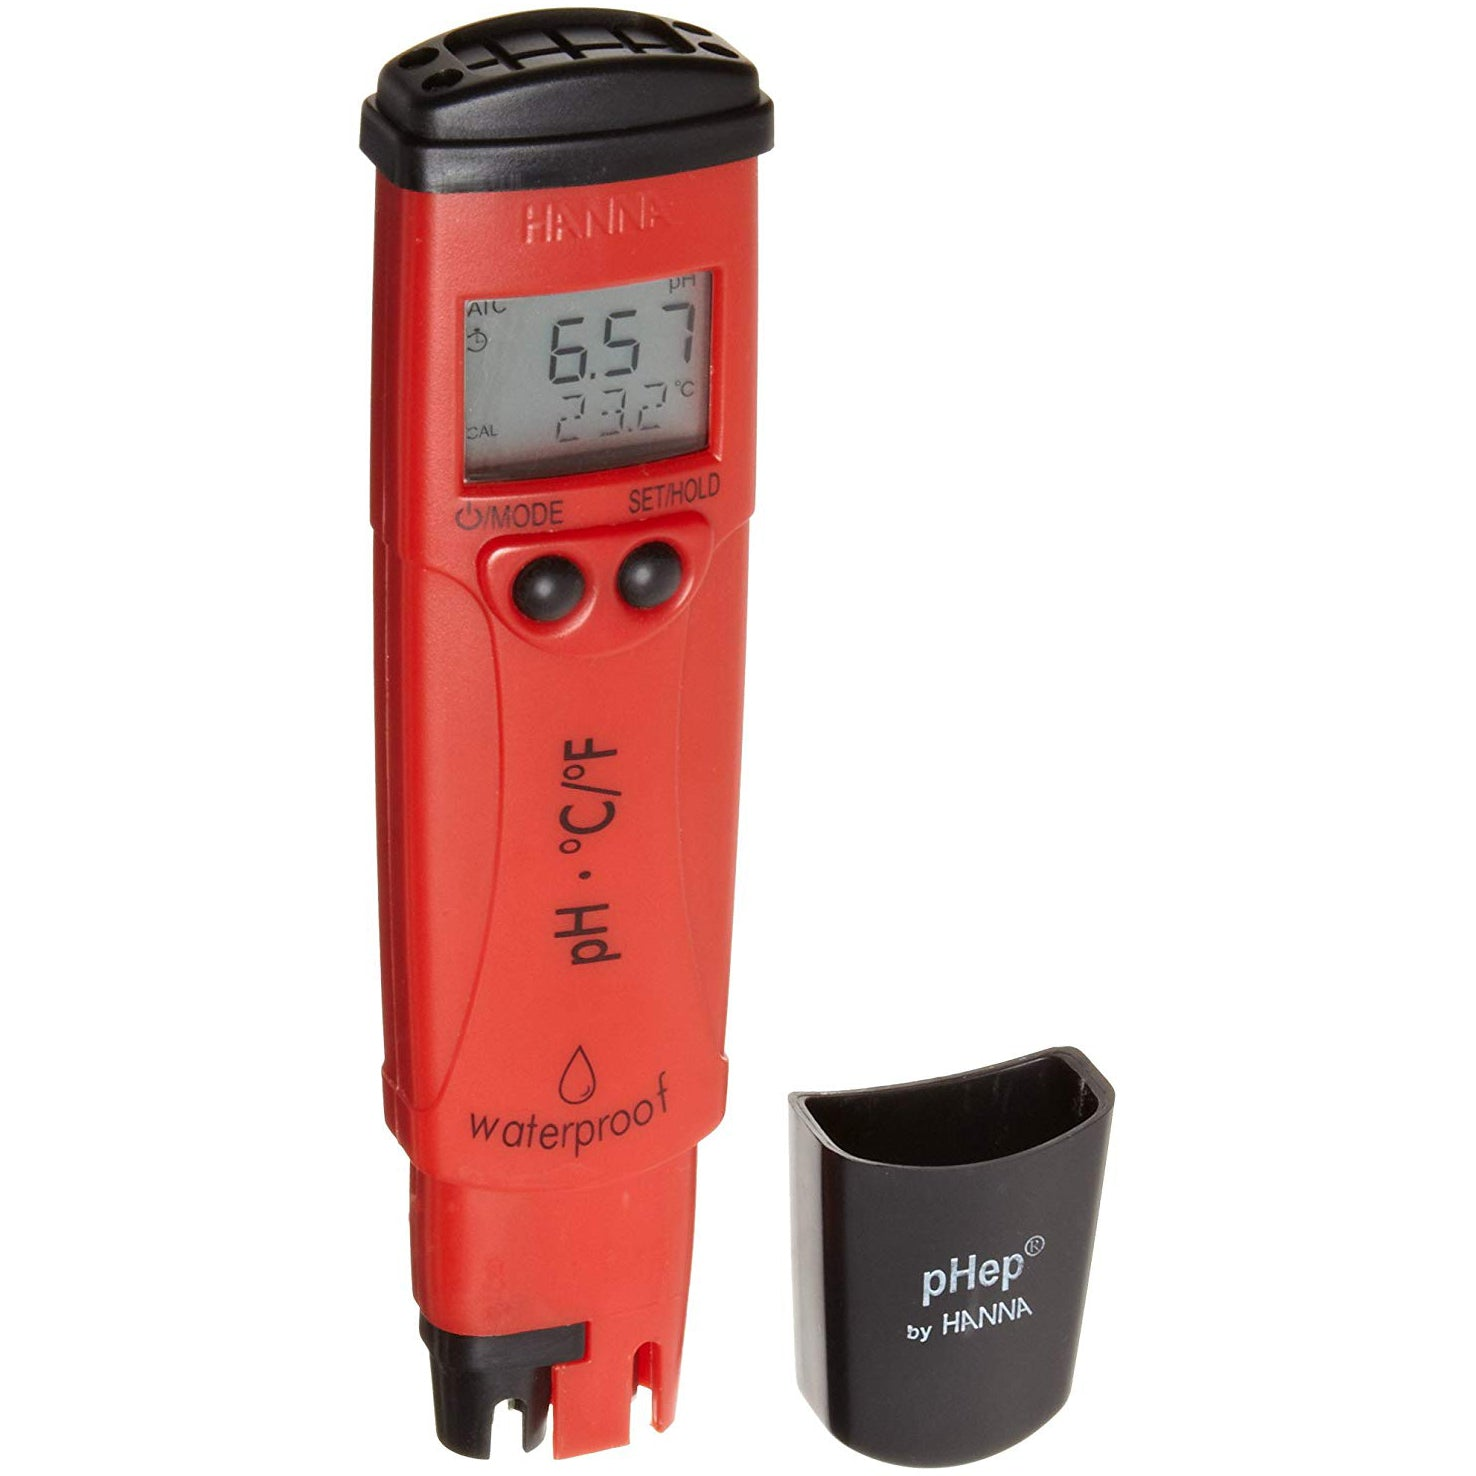
\includegraphics[width=\textwidth]{sensors/11_hanna.jpg}
    \caption{Hanna pHep \cite{hanna}}
  \end{minipage}
\end{figure}

\subsubsection{First solution}
The first solution is marked in pink. Both sensors repeatedly measured a pH of 4.4.

\begin{figure}[h]
  \centering
  \begin{minipage}[b]{0.2\textwidth}
    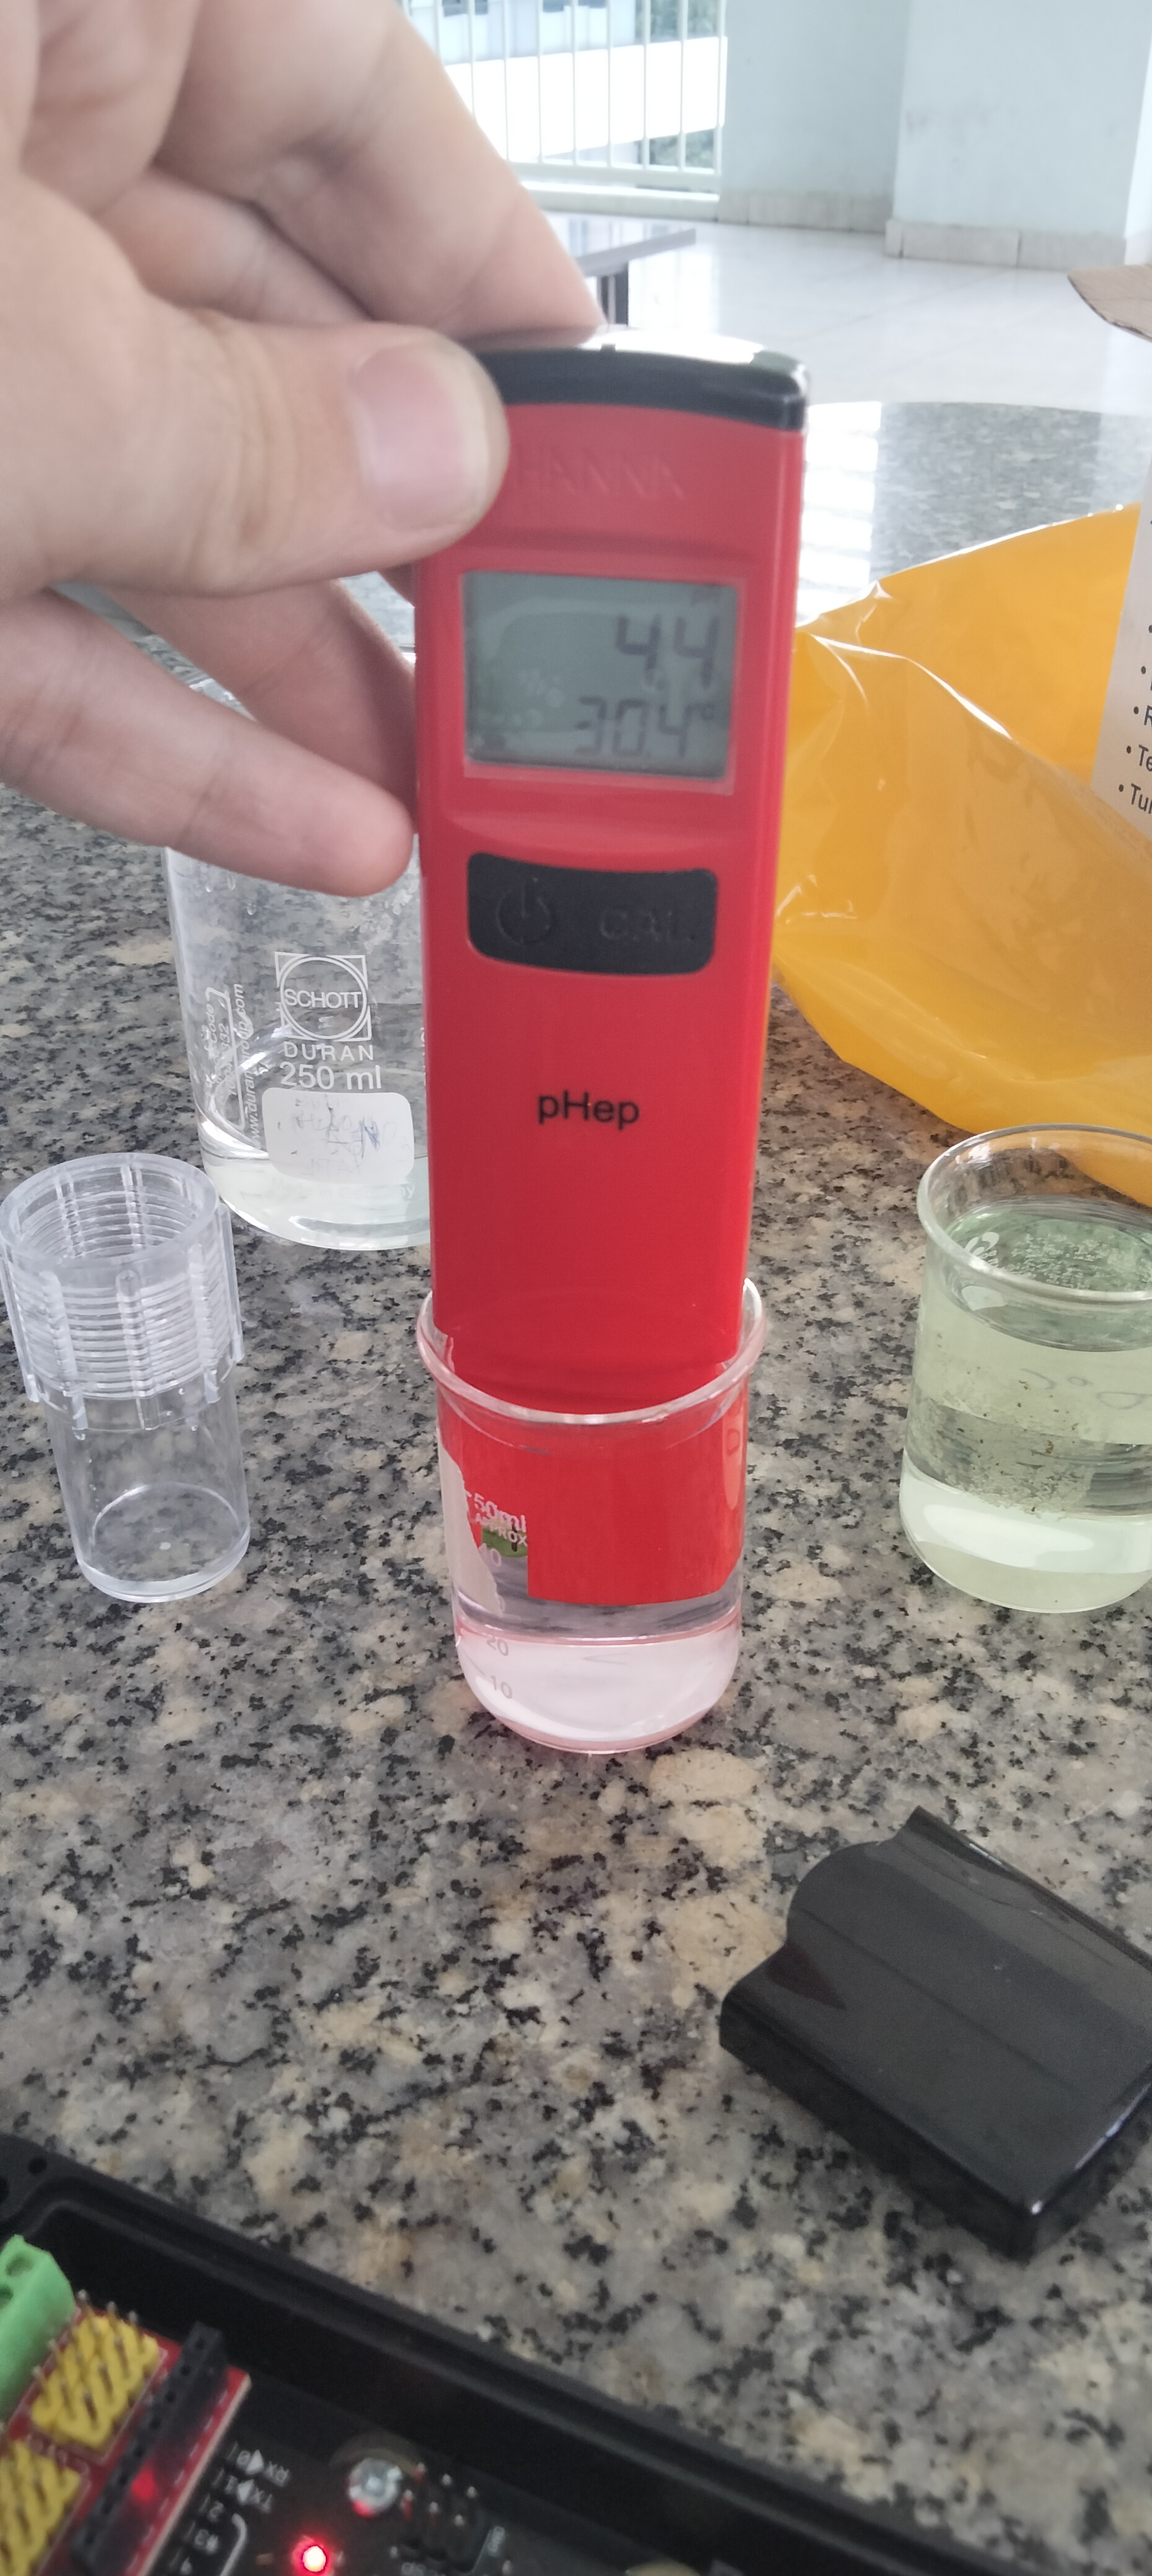
\includegraphics[width=\textwidth]{sensors/14_ph4_hanna.jpg}
    \caption{Hanna sensor measuring 4.4}
  \end{minipage}
  \hfill
  \begin{minipage}[b]{0.7\textwidth}
    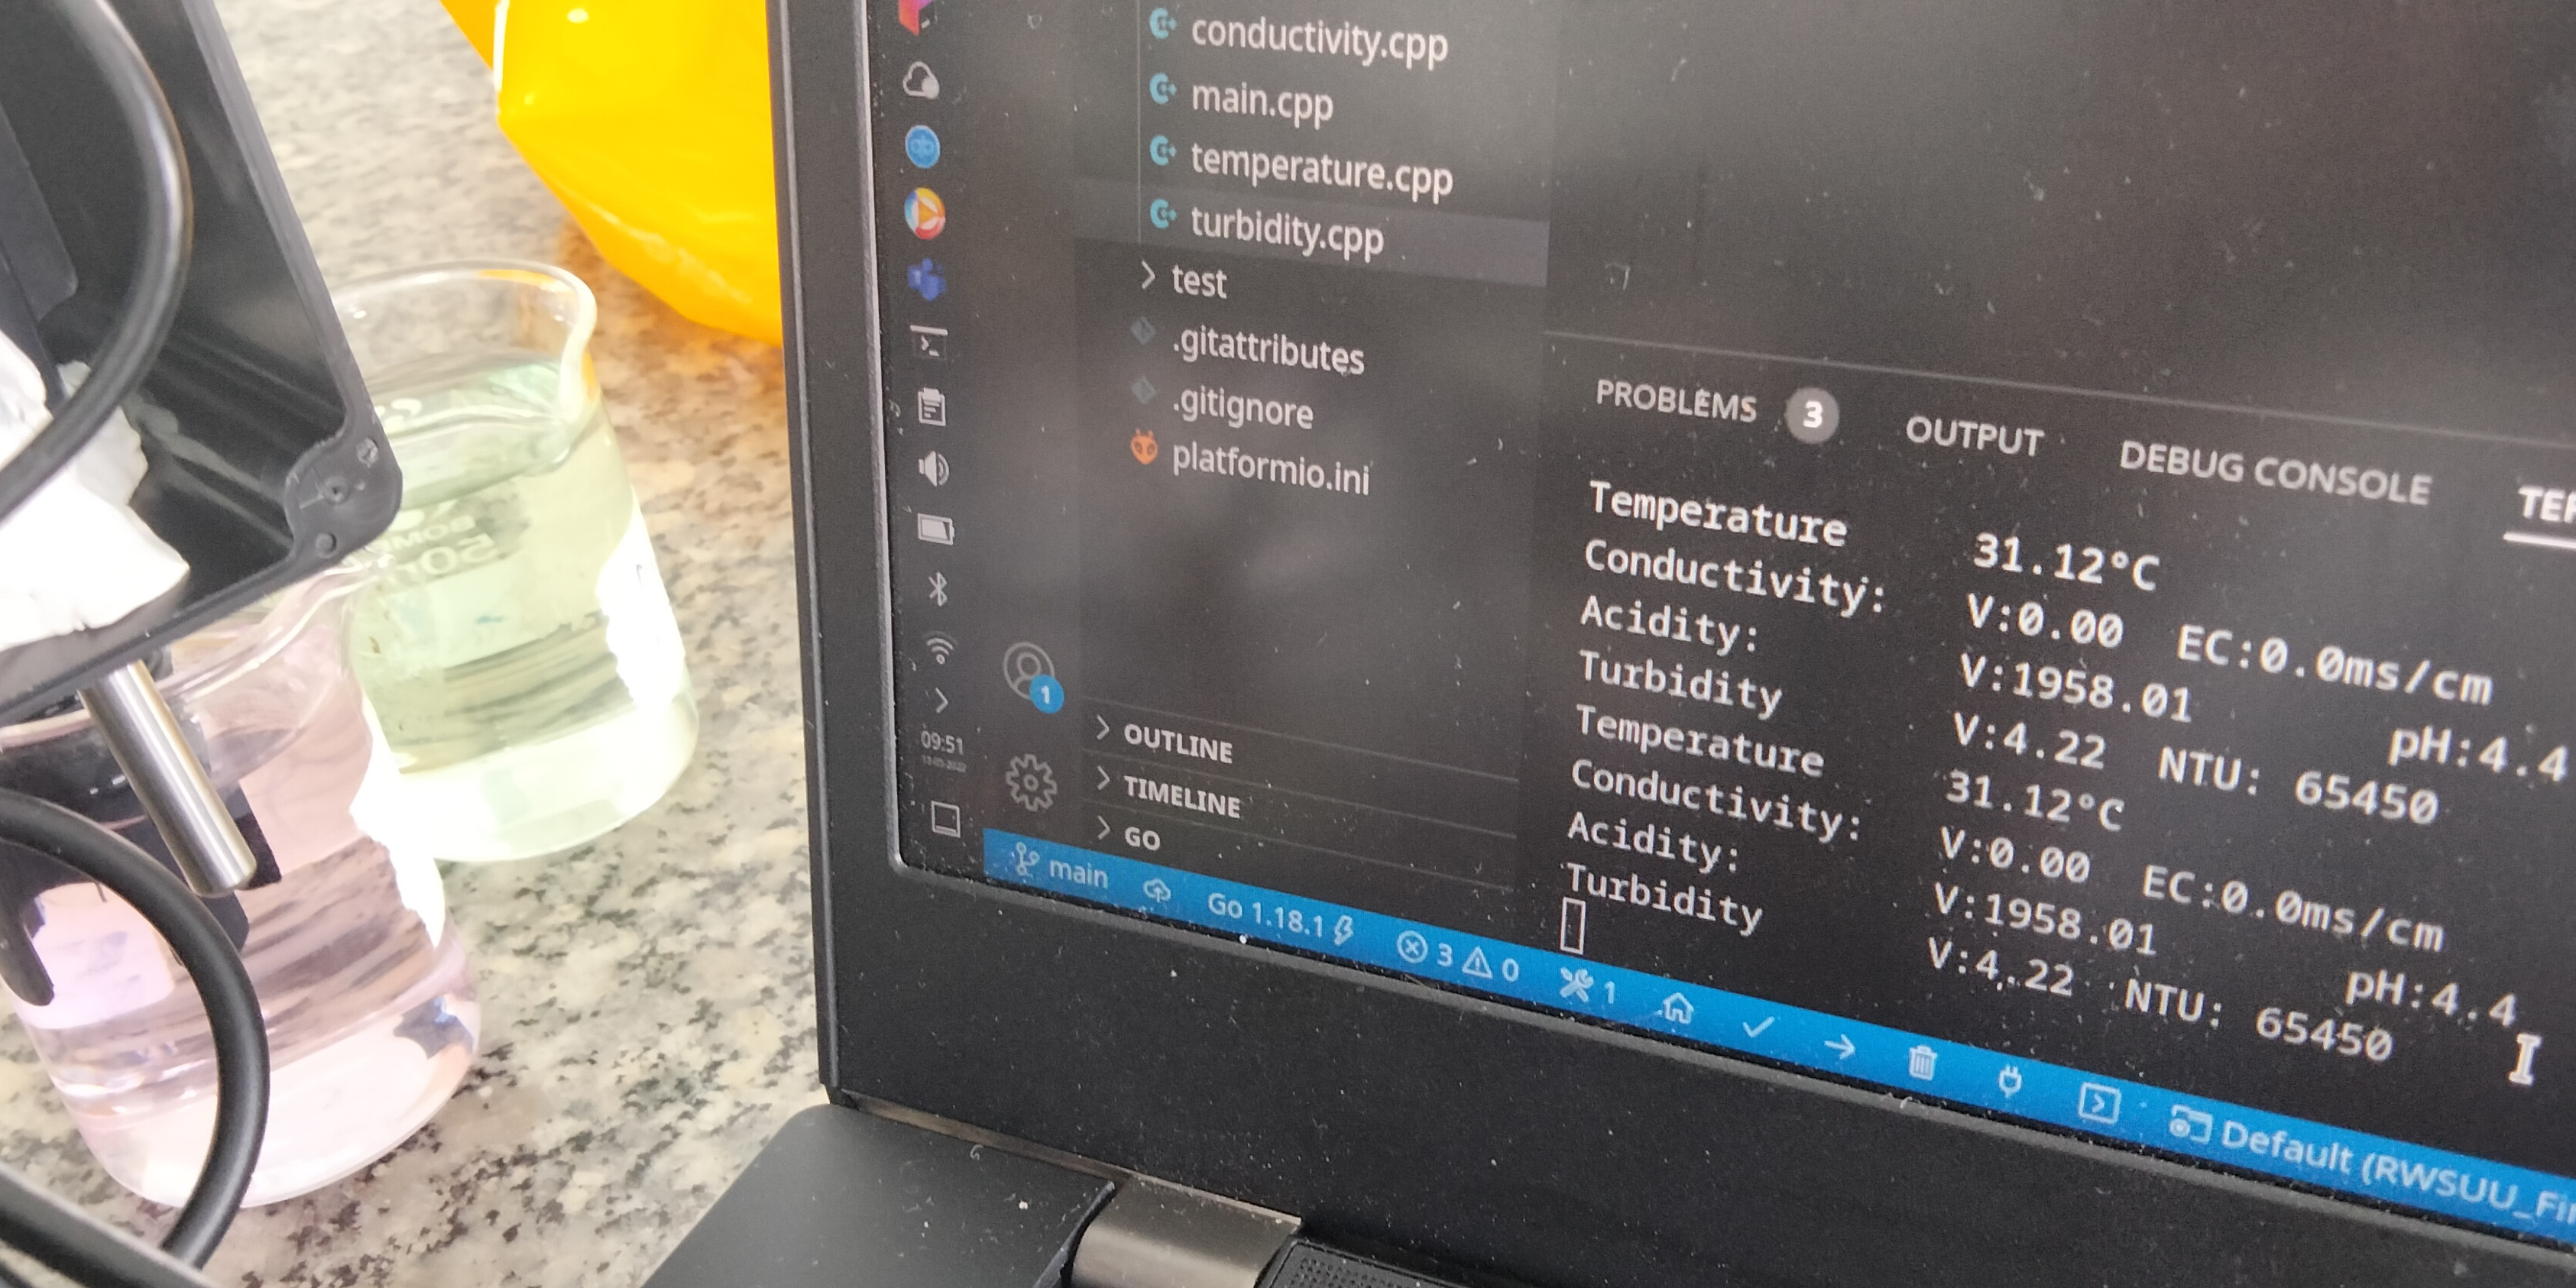
\includegraphics[width=\textwidth]{sensors/13_ph4_dfrobot.jpg}
    \caption{DFRobot sensor measuring 4.4}
  \end{minipage}
\end{figure}

\subsubsection{Second solution}
The second solution is marked in light yellow. The Hanna pHep repeatedly measured a pH of 7.2, while the DFRobot sensor repeatedly measured a pH of 7.3

\begin{figure}[h]
  \centering
  \begin{minipage}[b]{0.2\textwidth}
    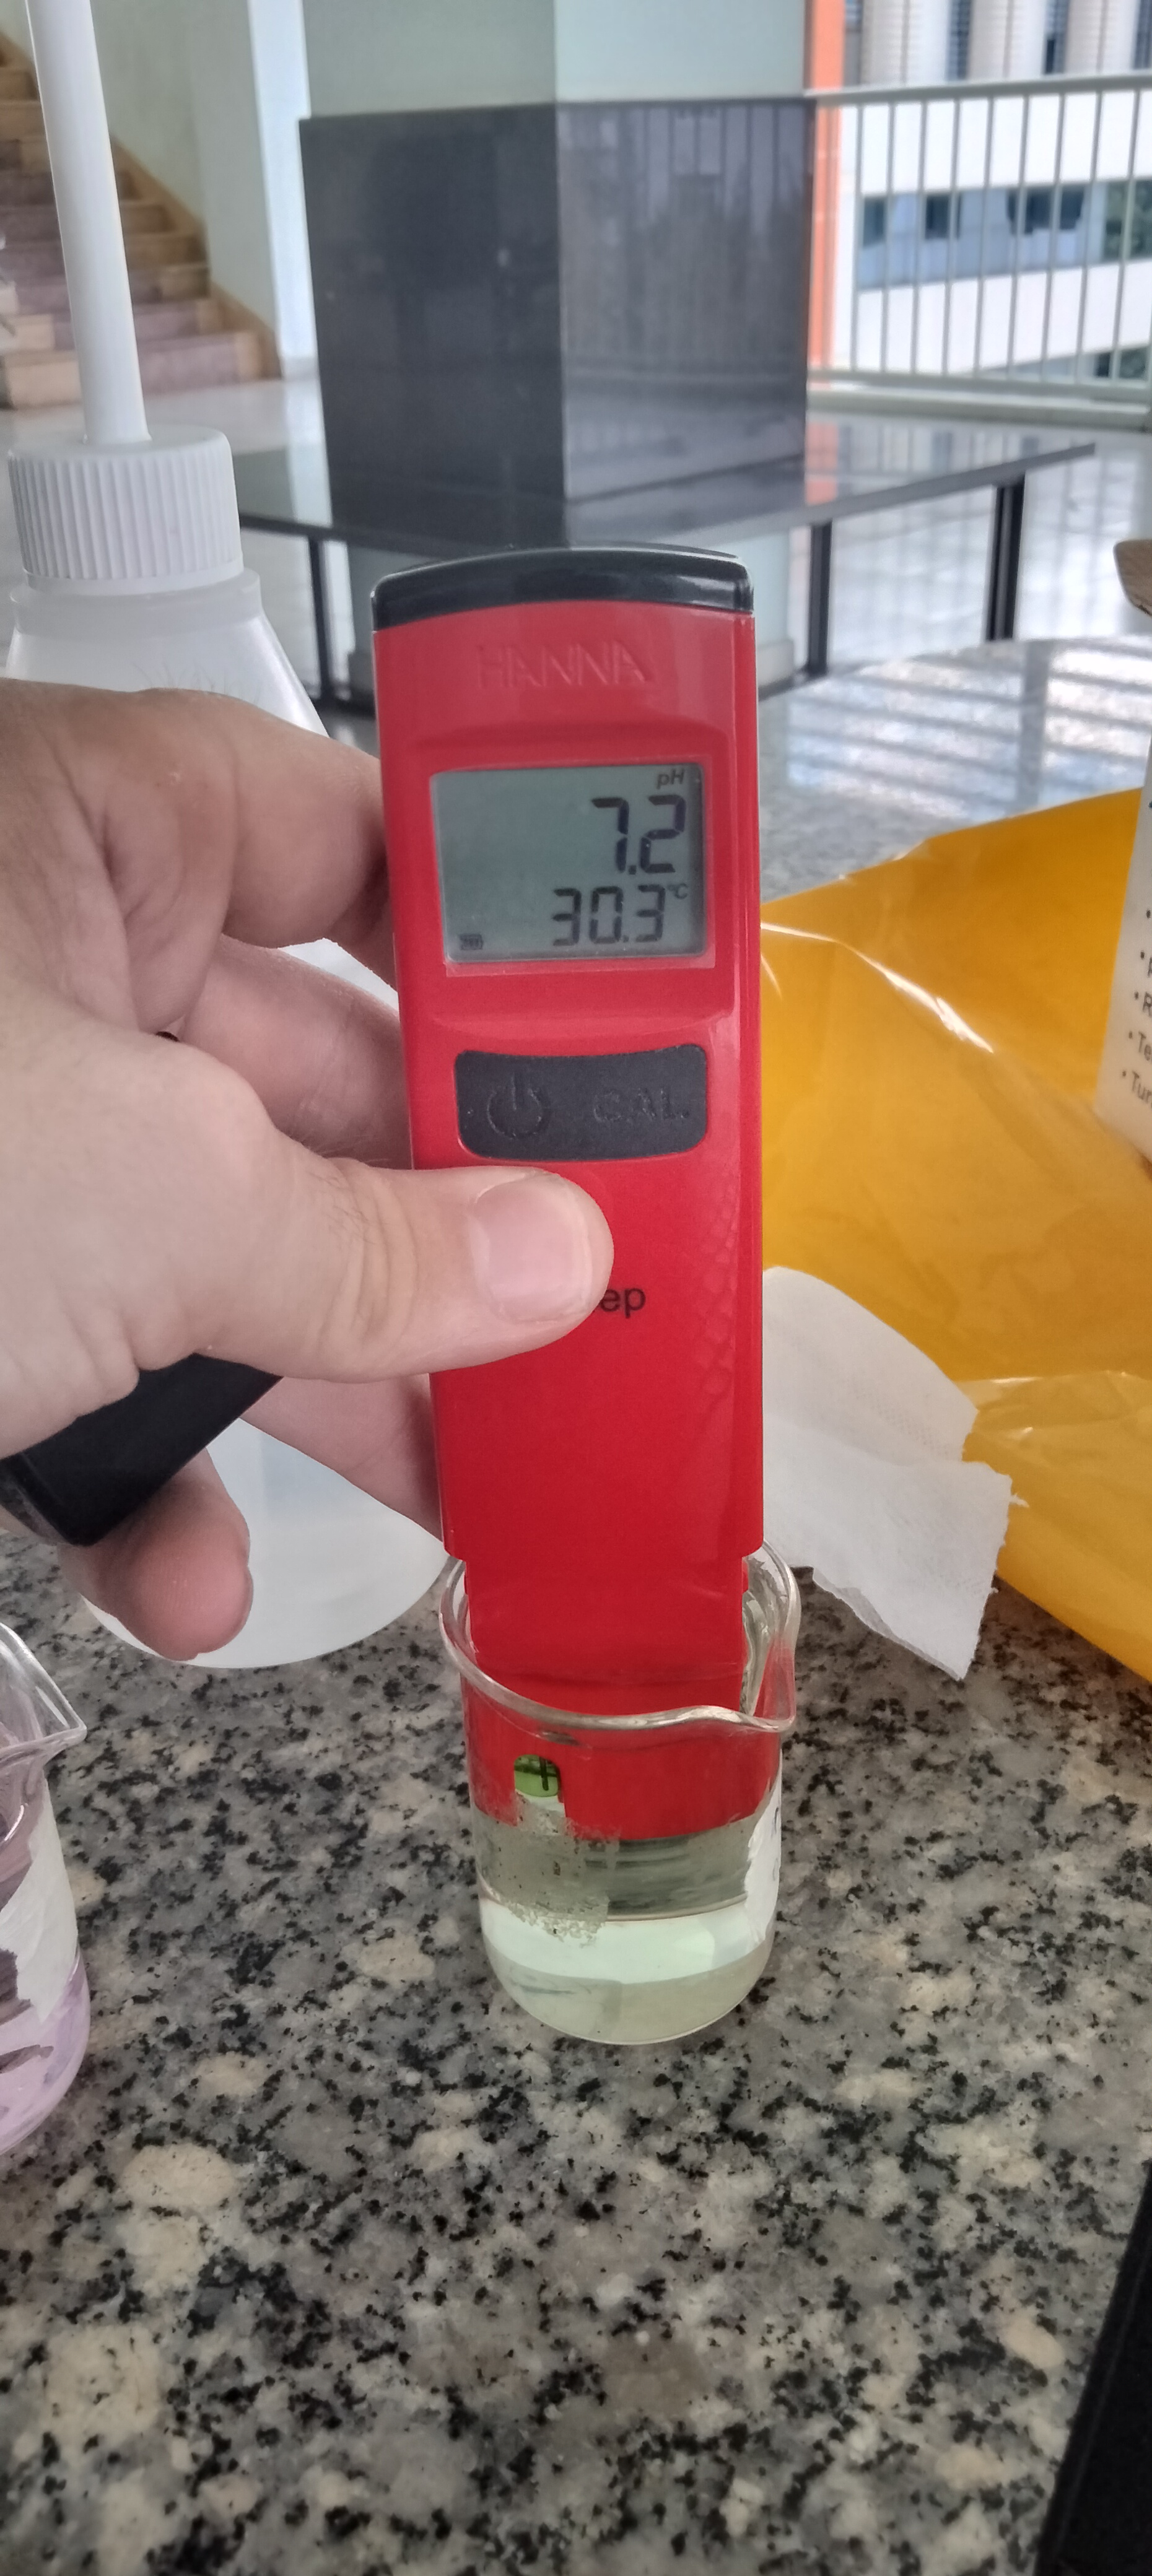
\includegraphics[width=\textwidth]{sensors/16_ph7_hanna.jpg}
    \caption{Hanna sensor measuring 7.2}
  \end{minipage}
  \hfill
  \begin{minipage}[b]{0.7\textwidth}
    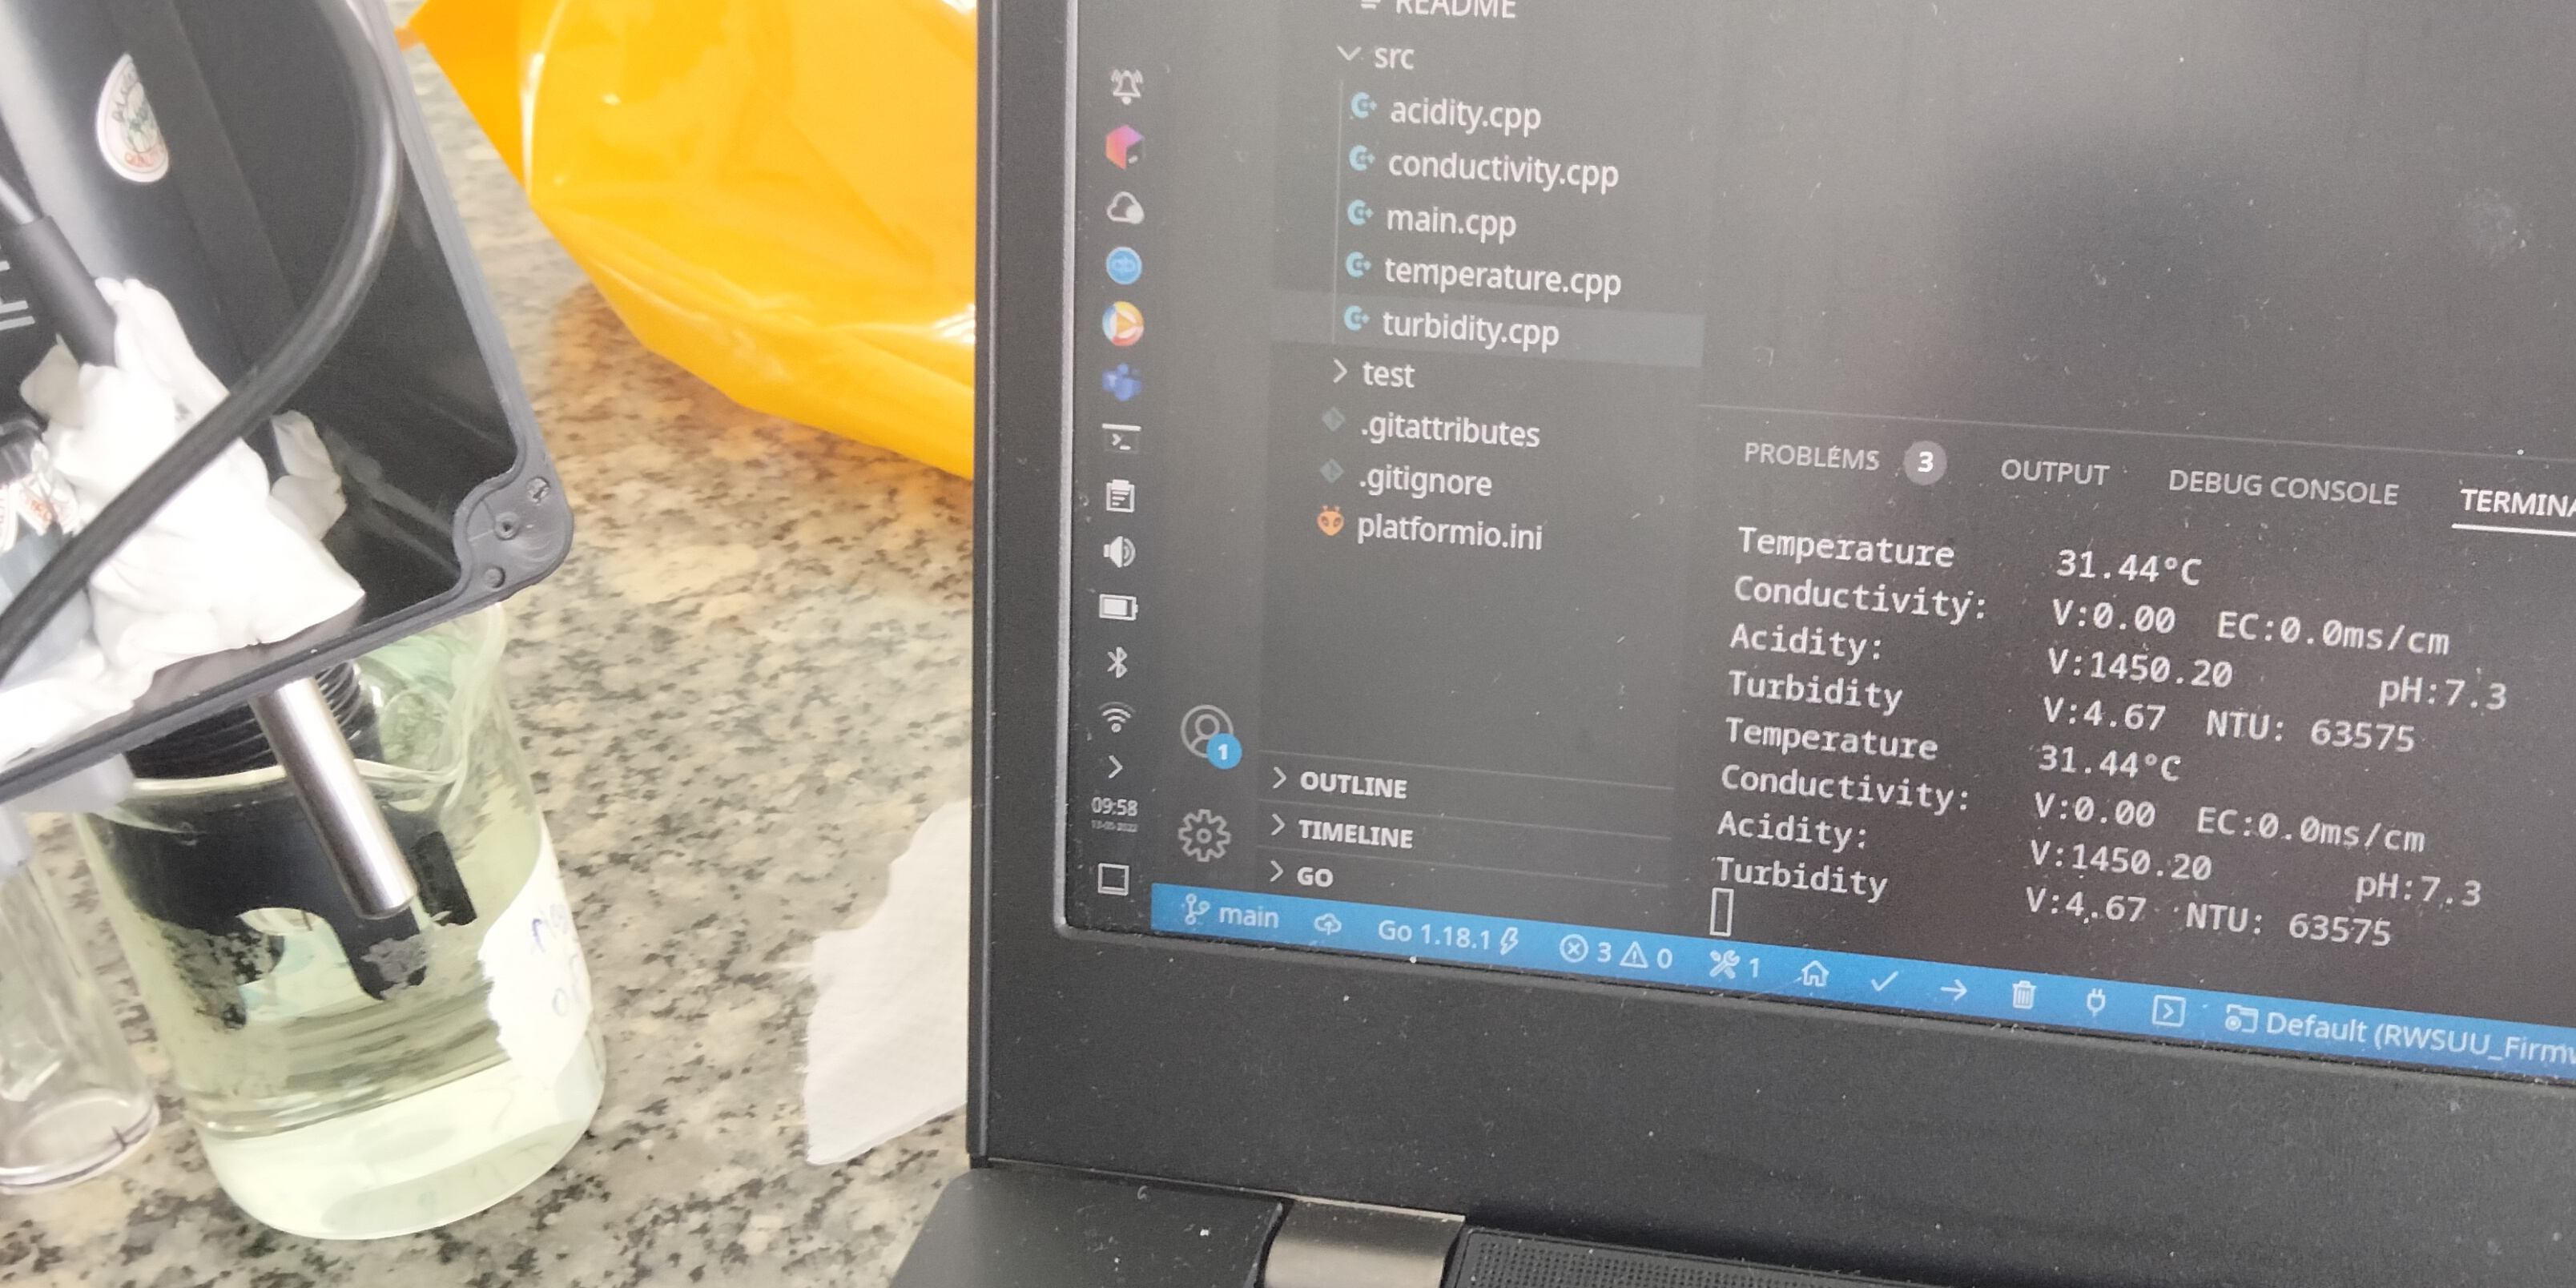
\includegraphics[width=\textwidth]{sensors/15_ph7_dfrobot.jpg}
    \caption{DFRobot sensor measuring 7.3}
  \end{minipage}
\end{figure}

\subsection{Conductivity}
As mentioned in the Design Report, the DFRobot DFR0300H \cite{DFR0300H} was chosen for measuring the conductivity. The manufacturer claims the sensor has an accuracy of 5\% FS, meaning with a range of 20ms/cm, it has an error of 1ms/cm. 

\begin{table}[h!]
	\centering
	\adjustimage{height=4cm,valign=c}{sensors/23_dfr0300h.jpg}\quad
	\begin{tabular}{| l | l |}
    \hline
    Protocol & Analog\\
    Measurement Accuracy &  5\% FSR\\
    Supply Voltage & 3.3-5V\\
    Support Detection Range & 10~100ms/cm\\
    Software library included & yes \\
    Probe included & yes \\
    Availability & 3-5 Working days \\
    \hline
	\end{tabular}
\end{table}

\subsubsection{Known conductivity solutions}
Known conductivity solutions of 12.88ms/cm and 1.413ms/cm were used to determine the accuracy of the sensor.

\begin{figure}[h]
  \centering
  \begin{minipage}[b]{0.7\textwidth}
    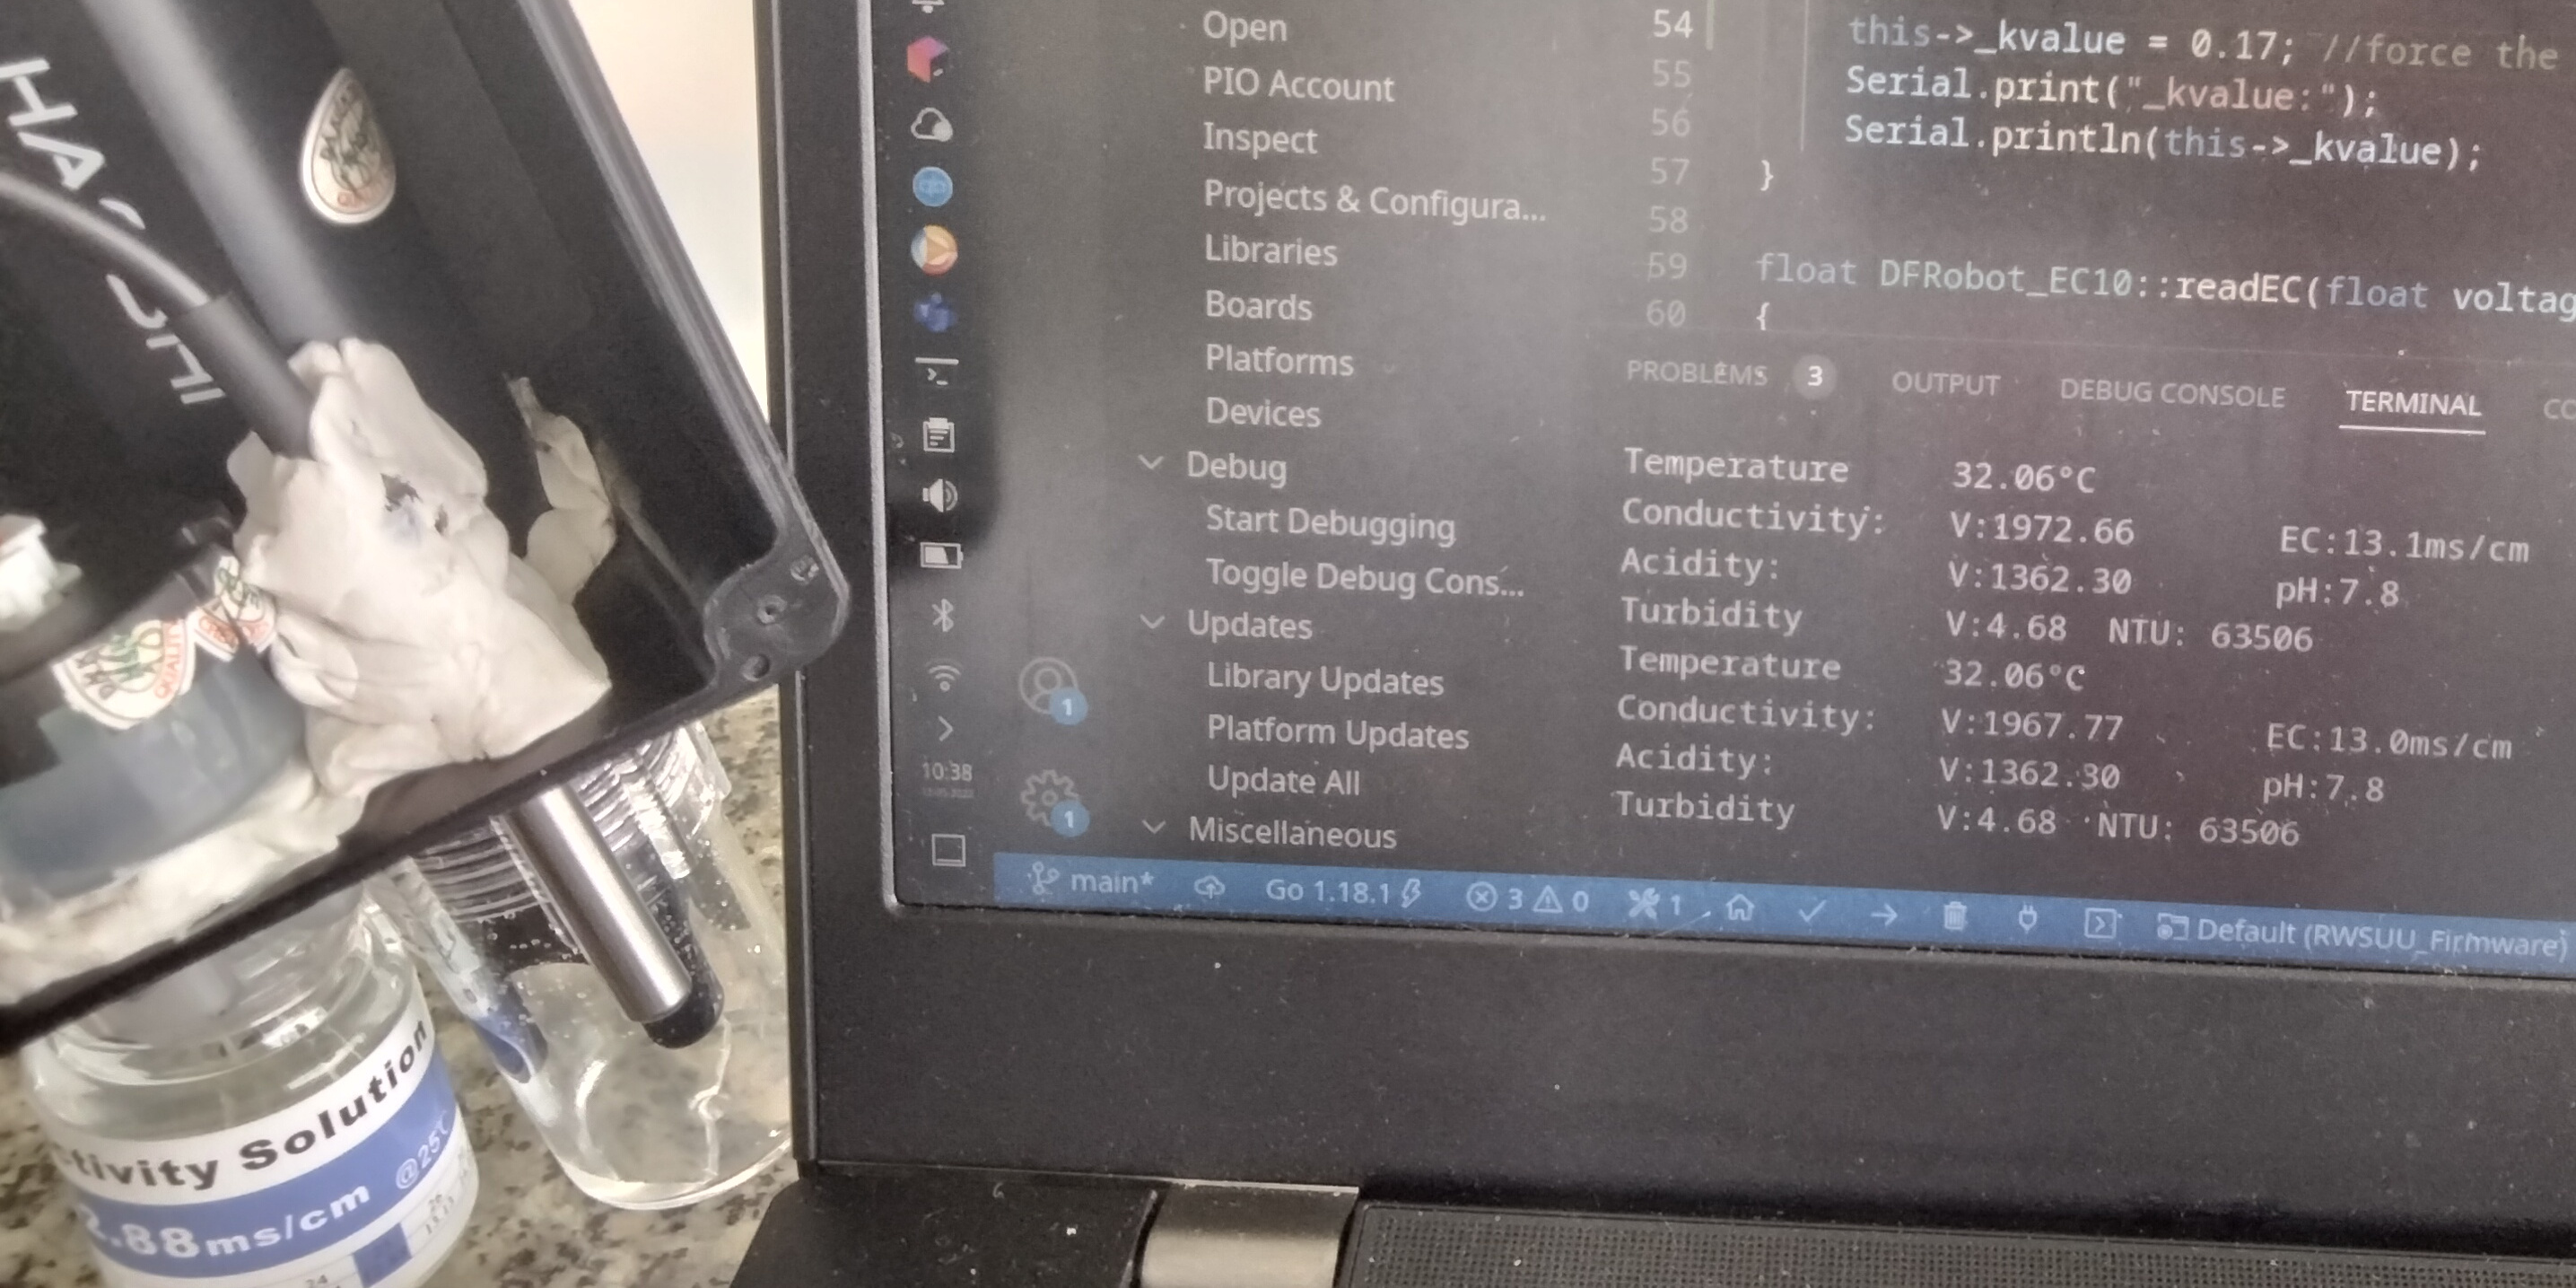
\includegraphics[width=\textwidth]{sensors/21_ec1288_dfrobot.jpg}
    \caption{measured 13.0 at 12.88ms/cm solution}
  \end{minipage}
  \hfill
  \begin{minipage}[b]{0.7\textwidth}
    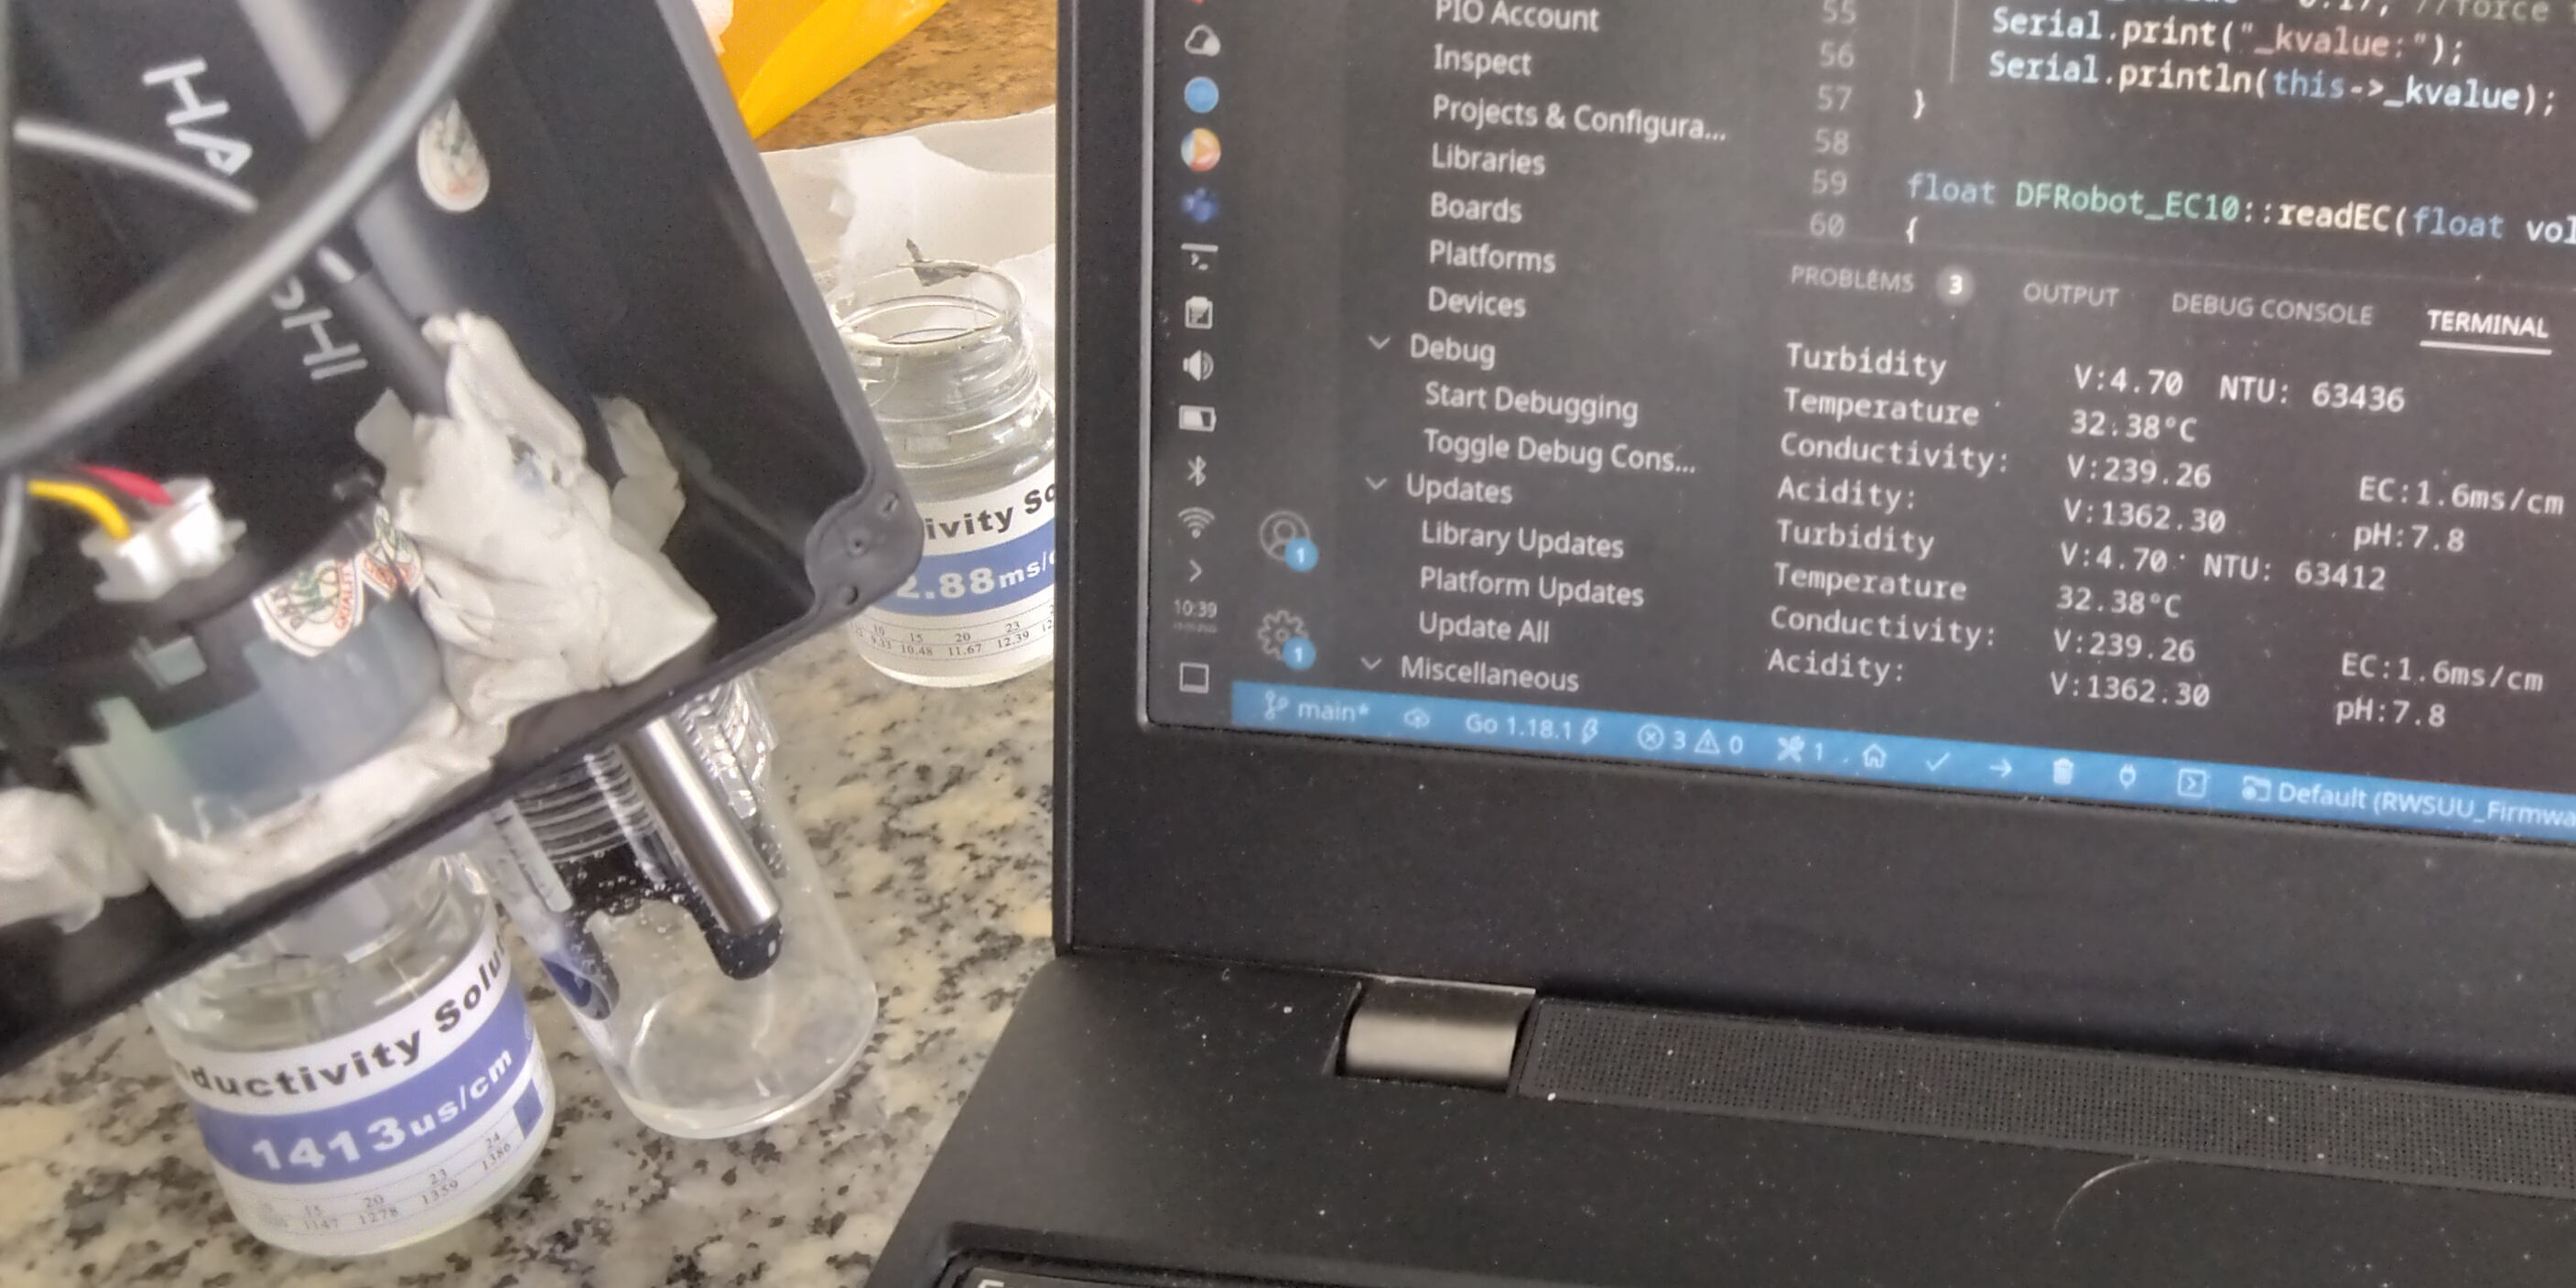
\includegraphics[width=\textwidth]{sensors/22_ec1413_dfrobot.jpg}
    \caption{measured 1.6 at 1.413ms/cm solution}
  \end{minipage}
\end{figure}
\subsection{Temperature}
As mentioned in the Design Report, the DFRobot DFR0198/DS18B20 \cite{DFR0198} waterproof sensor was chosen to measure the temperature. Temperature readings of the water are both recorded and used to help determining the acidity and conductivity.

\begin{table}[h!]
	\centering
	\adjustimage{height=4cm,valign=c}{sensors/31_dfr0198.jpg}\quad
	\begin{tabular}{| l | l |}
    \hline
    Protocol & 1-Wire\\
    Measurement Range & -10-85 ℃ \\
    Measurement Accuracy &  0.5 ℃ \\
    Response time & Within 750ms \\
    Supply Voltage & 3.3V-5V \\
    Software library included & yes \\
    Availability & 3-5 Working Days \\
    \hline
	\end{tabular}
\end{table}



\pagebreak
\printbibliography 

\end{document}